%%%%%%%%%%%%%%%%%%%%%%%%%%%%%%%%%%%%%%%%%%%%%%%%%%%%%%%%%%%%%%%%%%%
%                                                                 %
%  GEANT manual in LaTeX form                                     %
%                                                                 %
%  Michel Goossens (for translation into LaTeX)                   %
%  Version 1.00                                                   %
%  Last Mod. Jan 24 1991  1300   MG + IB                          %
%                                                                 %
%%%%%%%%%%%%%%%%%%%%%%%%%%%%%%%%%%%%%%%%%%%%%%%%%%%%%%%%%%%%%%%%%%%
\Origin{I.Gavrilenko, P.Nevski, K.Lassila-Perini}
\Documentation{K.Lassila-Perini}
\Version{Geant 3.21}\Routid{PHYS334}
\Submitted {11.03.94}\Revised{11.03.94}
\Makehead {Models for energy loss fluctuations in thin layers}

\section{Subroutines}

\Shubr{GSTINI}{}
\Rind{GSTINI} initializes the tables that are used for sampling of
the energy loss, if the user has set the flag {\tt STRA = 1}.
It calls the subroutine \Rind{GSTXIN} to integrate
an expression for the number of collisions and \Rind{GSTTAB}
for preparing the tables for different Lorentz factors.
It is called from \Rind{GPHYSI} at initialization time.

\Shubr{GSTXIN}{}
\Rind{GSTXIN} computes the values needed for the sampling tables.
It uses the functions \Rind{GOSCIN} to integrate over the
photoelectric cross-sections and the function \Rind{GKOKRI}
to compute the real part of the complex dielectric constant.
\Rind{GSTXIN} is called from \Rind{GSTINI}.

\Sfunc{GOSCIN}{VALUE = GOSCIN(EIN1EV,EIN2EV)}
\Rind{GOSCIN} integrates the parameterization of the photoelectric
cross-sections from energy {\tt EIN1EV} to energy {\tt EIN2EV}.
It is called from \Rind{GSTXIN}.

\Sfunc{GKOKRI}{VALUE = GKOKRI(E,EMINEV,EMAXEV)}
\Rind{GKOKRI} computes the real part of the complex dieletric
constant which is needed in the preparation of energy loss
sampling tables. {\tt E} in the energy for which the values
are being tabulated, {\tt EMINEV} and {\tt EMAXEV} are
the integration limits. \Rind{GKOKRI} is called from
\Rind{GSTXIN}.

\Shubr{GSTTAB}{(GAM,NT,EN,FN)}
\Rind{GSTTAB} prepares the energy loss sampling tables for
different Lorentz factors. The input {\tt GAM} is the Lorentz factor,
the output values are: {\tt NT} the lenght of the table,
{\tt EN} the energy array and {\tt FN} the cumulative probabilty array.
It calls \Rind{GXGINT} to integrate over the probability
function \Rind{GSTDN} to
get the value of {\tt FN}. \Rind{GSTTAB} is called from
\Rind{GSTINI}.

\Sfunc{GXGINT}{VALUE = GXGINT(EXT,A,B,EPS)}
\Rind{GXGINT} performs the Gaussian integration from {\tt A} to
{\tt B} over the function {\tt EXT} with accuracy {\tt EPS}.
It is called from \Rind{GSTTAB} to integrate over the probability
function \Rind{GSTDN}.

\Sfunc{GSTDN}{VALUE = GSTDN(LGE)}
\Rind{GSTDN} is the function which gives the probability for a collision
with energy transfer {\tt LGE}. It is integrated to get the
cumulative probabilty function to be used in the sampling
of the energy loss.

\Shubr{GSTREN}{(GAMMA,ECUT,STEP)}
\Rind{GSTREN} computes the energy loss for a particle of
Lorentz factor {\tt GAMMA} in a step of length {\tt STEP}
if the user has set the flag {\tt STRA = 1}.
{\tt ECUT} is the cut for the $\delta$-ray production.
\Rind{GSTREN} is called from \Rind{GFLUCT}.

\section{The method}
In thin layers, the Landau model of energy loss fluctuations
is not valid, because the number of collisions is too small.
In this case, the atomic structure of the atom has to be
taken into account. The photoabsorption ionization
(PAI) model uses the photoelectric cross-sections
to describe the energy loss distribution.
The results (the width and the most probable value of
the energy loss distribution function)
given by this model are equal to those given by
standard {\tt GEANT} procedure described in {\tt [PHYS332]}.
In addition, however, it gives an estimate of the number
of collision in each step ({\tt NICOLL} in the common block
{\tt GCSTRA}). PAI model is slower than the standard
{\tt GEANT} method.

PAI model is activated, if the user set the flag
{\tt STRA = 1}. The default value is 0.

\subsection{The photoabsorption ionization model}
An expression for the distribution of energy loss can be derived
considering the energy loss as the sum of the energy transfers in
the electromagnetic interactions between
the particle and the atom.
As the interaction is small (i.e. the energy transfer is
small compared to the energy of the passing particle),
Born approximation can be used in the perturbation theory.
In the derivation, the atomic transition current is
considered as a sum of the transition currents of its
electrons.


$\varepsilon$ is the complex
dielectric constant of a medium which describes the
electromagnetic properties of
the medium and thus the effect of the field of an atom
on the energy loss of the particle.

The complex dielectric constant can be written $\varepsilon =
\varepsilon_1 + i \varepsilon_2$ where $\varepsilon_1$ describes
the polarization and $\varepsilon_2$ the absorptive properties
of the medium. $\varepsilon_2$ can be expressed with the
help of the oscillator strength function $f(k,\omega)$ which
describes the coupling of the electrons to the field of the
atom.
\begin{equation}
\label{eps2}
\varepsilon_2 = \frac{2 \pi^2 N e^2}{m \omega} f(k,\omega)
\end{equation}
$m$ is the mass of the electron and $N$ is the electron density.
In a simplified model, the photoabsorption cross-section
$\sigma_{\gamma}(\omega)$ can be used for description of $f(k,\omega)$:
\begin{equation}
f(k,\omega) = \frac{mc}{2\pi^2 e^2 Z} \sigma_{\gamma}(\omega)
\end{equation}
$Z$ being the atomic number of the medium.
The real part of $\varepsilon$ can be  expressed as an integral
of the imaginary part according to the Kronig's and Kramers' dispersion
relation\cite{bib-ALLIS}:
\begin{eqnarray}
\varepsilon_1 - 1 & = & \frac{2}{\pi} P \int_0^{\infty}
     \frac{x \varepsilon_2(x) dx}{x^2 - \omega^2} \nonumber \\
                  & = & \frac{2 N c}{\pi Z} P \int_0^{\infty}
     \frac{\sigma_{\gamma}(x) dx}{x^2 - \omega^2}
\label{eps1}
\end{eqnarray}
where $P$ indicates the Cauchy principal value.
Using these assumptions for the interaction between the projectile
and the atom, the
following form is obtained for the collision cross-section \cite{bib-GRISH}:
\begin{eqnarray}
\frac{d\sigma}{dE}     & = & - \frac{e^2}{\pi \hbar^2c^2n_a}
    \mbox{ Im} \left[ \left( \frac{1}{\beta^2\varepsilon} - 1 \right)
              \ln \frac{2mv^2}{E(1-\beta^2\varepsilon)} \right] \nonumber \\
& &  + \frac{2\pi Ze^4}{mv^2E^2} \int_0^{\infty}
    \frac{f(E')}{\varepsilon(E')^2} dE'
\label{xsection}
\end{eqnarray}
where $n_a$ is the number of atoms per cm$^3$, $v$ velocity of the particle,
and $\beta=v/c$. The number of collisions per distance $x$ and
the energy $E$ is then
\begin{equation}
\frac{N^2}{dx dE} = n_a \frac{d\sigma}{dE}
\end{equation}

For the simulation purposes, the number of primary collisions
in a unit length
with energy loss greater than a certain E
is computed and tabulated for several values of the Lorentz factor.
This is done by integrating
\begin{eqnarray}
\left( \frac{dN}{dx} \right)_{>E}
& = &\int_E^{E_{max}} n_a \frac{d\sigma}{dE} dE
\label{integ}
\end{eqnarray}

\subsection{Implementation}
A photoabsorption ionization Monte Carlo code provided to us by users
%\cite{trd}
has been implemented in {\sc GEANT}. Tables are
prepared at initialization time and sampling from these
tables is done each step at running time. An important
thing to note is the dependence of the $(dN/dx)_{>E}$
on the photoelectric
cross-sections which, when taken from different sources,
may differ considerably, especially at low energies.

To fill the tables, the integration of equation \ref{xsection}
has to be done.
Before the integration over the energy, the integral
over
the oscillator strength function $f(k,\omega) \sim
\sigma_{\gamma}(\omega)$ (last term in equation \ref{xsection})
and the dielectric constant (equations \ref{eps1} and \ref{eps2})
$\varepsilon$ have to be computed. These integaration
can be done analytically when the parameterized cross-sections
are used.

The oscillator strength function should
fulfill the Bethe sum rule \cite{bib-BETH}:
\begin{equation}
\int_0^{\infty} f(k,\omega) d\omega = 1
\label{sumrule}
\end{equation}
To respect this condition, in the PAI model, one has to add some
contribution from the excitation processes to low-energy region
of the photoelectric cross-sections \cite{bib-ALLIS}. In {\sc GEANT}, the
photoelectric cross-section
parameterization of the Sandia \cite{bib-SANDIA} report is used.
In order not to change the tabulated parameterization, the sum
rule is taken into account by lowering the energy
limit for the integration below the ionization limit.
This will not satisy the equation \ref{sumrule} in all cases.
In the program, however, the Bethe sum rule is forced by
dividing the integrated cross-section from $E$ to $\infty$
by the value given by the integration over the whole range.
\begin{figure}[t]
   \centering
   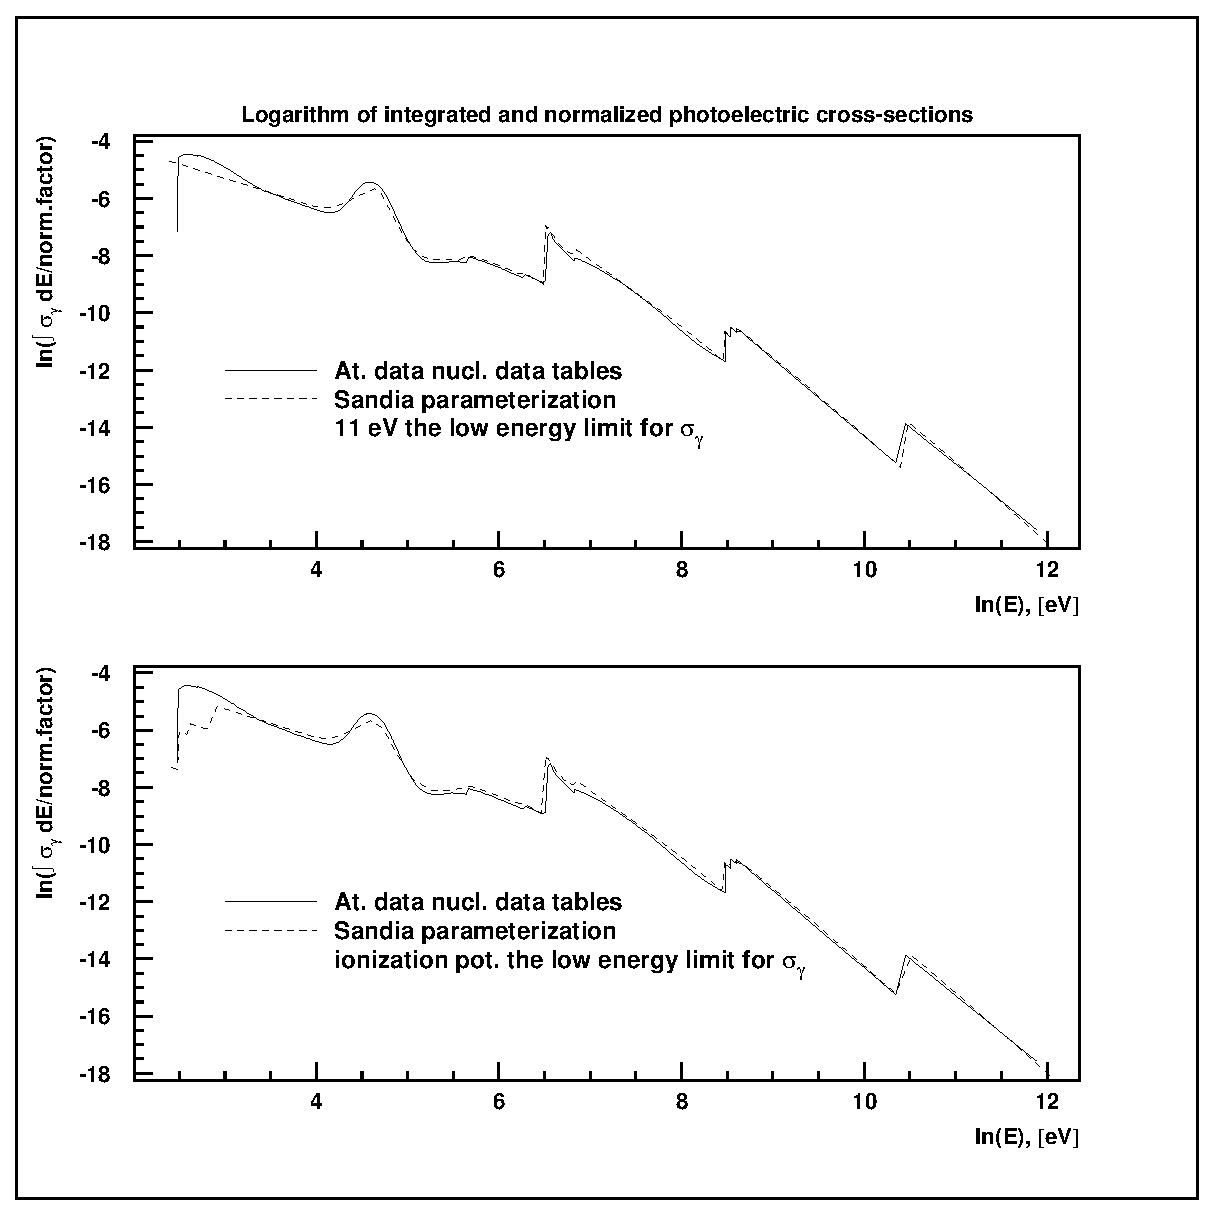
\epsfig{file=eps/phys334-1.eps,width=10cm}
   \caption{Above, the integrated and normalized cross-section
    of the gas mixture 70\% Xe - 10\% CO$_2$ - 20\% CF$_4$
    for two different data sets. The low energy limit
    of the cross-sections from the Sandia data in chosen
    to be 11 eV. In the figure below, the low energy limit
    is the ionization limit for each component of the mixture}
    \label{fosc}
\end{figure}
In figure \ref{fosc}, the integrated cross-section (oscillator
strength function)
$\int_{E}^{E_{max}} \sigma_{\gamma} / \int_{E_0}^{E_{max}} \sigma_{\gamma}$
is given for two different sets of photoelectric cross-section
data for a gas mixture 70\% Xe - 10\% CO$_2$ - 20\% CF$_4$.
In the figure below, the continuous line is the result of the
integration tabulated from \cite{bib-ATOM1} \cite{bib-ATOM2} \cite{bib-ATOM3} 
and the dashed line
is from the integration of {\sc GEANT} cross-sections
considering the lower limit of the cross-section the ionization
energy (12.3 eV for Xe, 11.26 eV for C, 13.6 for O, and
17.42 for F).
In the figure above, the continuous line is as before, but for
the dashed line, the lower limit of the cross-sections is
considered to be 11 eV for all elements of the mixture
to compensate for the sum rule.

The imaginary part of the complex dielectric constant can then
be computed from the integrated cross-section.
To compute the real part of $\varepsilon$, one needs to take the
Cauchy principal value which is basically a limiting process
cancelling the two infinite contribution around the pole
$(x_0-\delta,x_0+\delta)$. The derivation of the real part
with the Sandia parametrization is shown in detail
in the appendix.
\begin{figure}[t]
   \centering
   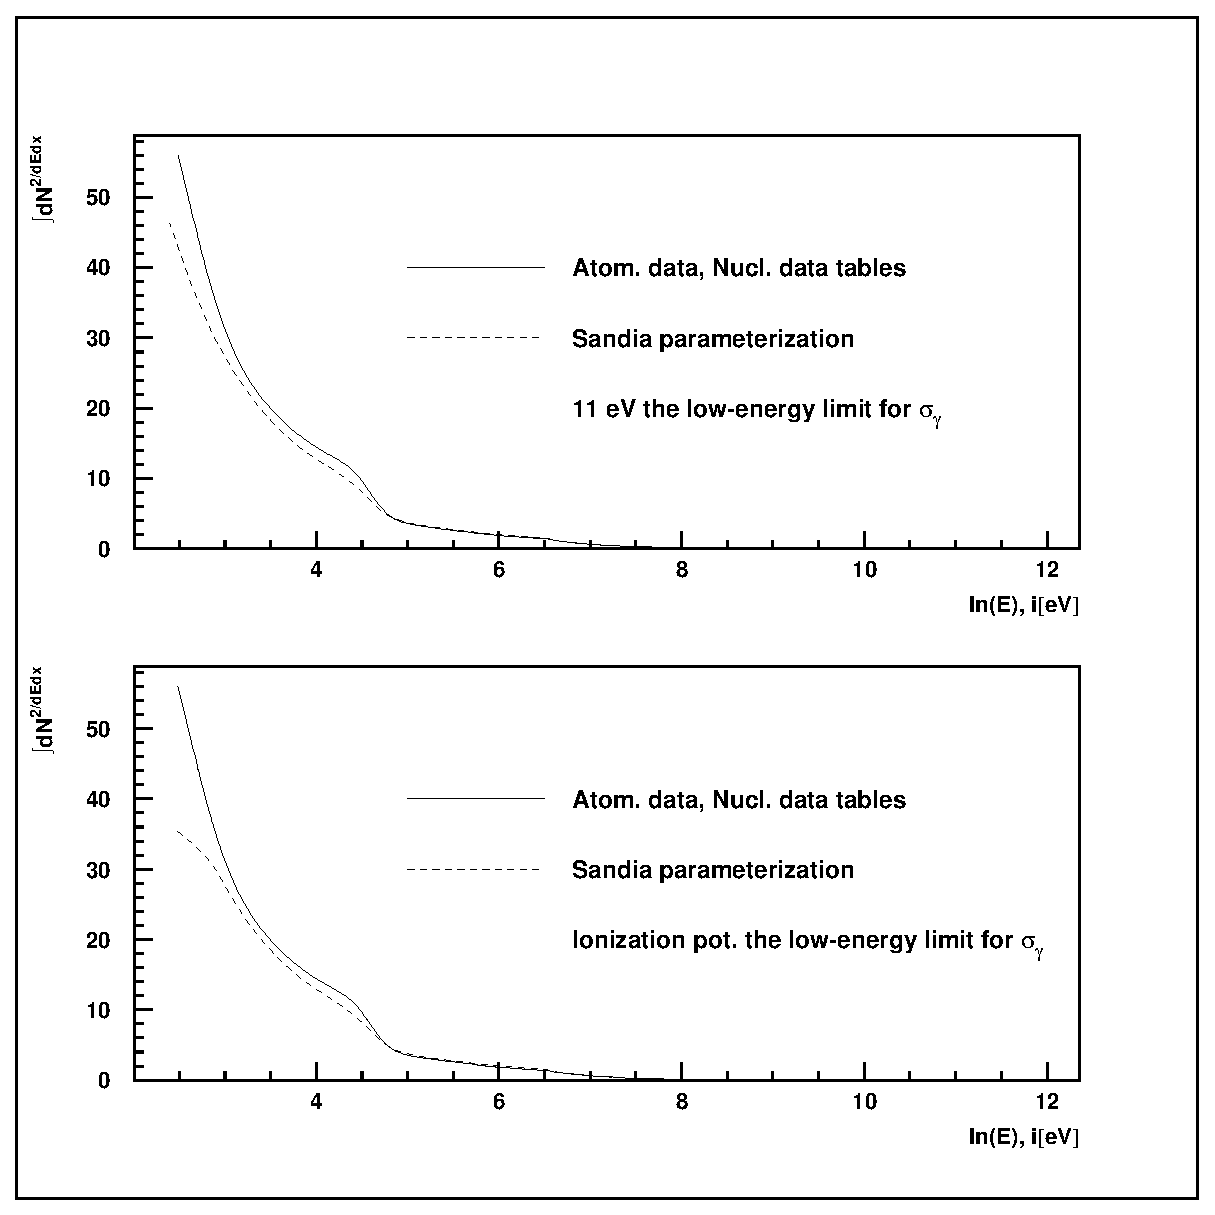
\epsfig{file=eps/phys334-2.eps,width=10cm}
   \caption{Above, the integrated and normalized cross-section
    of the gas mixture 70\% Xe - 10\% CO$_2$ - 20\% CF$_4$
    for two different data sets. The low energy limit
    of the cross-sections from the Sandia data in chosen
    to be 11 eV. In the figure below, the low energy limit
    is the ionization limit for each component of the mixture}
    \label{idndx}
\end{figure}

Knowing the values of complex dielectric constant and the integrated
cross-section, the integration of equation \ref{integ} can
be done. This is done for several values of Lorentz factor
during the initialization time in  subroutine {\tt GSTINI}.
The value of energy loss is sampled from these tables in
subroutine {\tt GSTREN}.

One should remember the dependence of this method on the
photoelectric cross section data.
Figure \ref{idndx} shows the results for the two different
data sets. The difference in the low-energy part is very
significative as the sampling is done from these tables
and, according the inverse transverse method, the number of
collisions is sampled between the maximum and minimum
of the curves in figure \ref{idndx}.








